\documentclass[tikz,10pt]{standalone}

\definecolor{cccanard}{RGB}{4,139,154}
\definecolor{cccitrouille}{RGB}{223,109,20}

\begin{document}
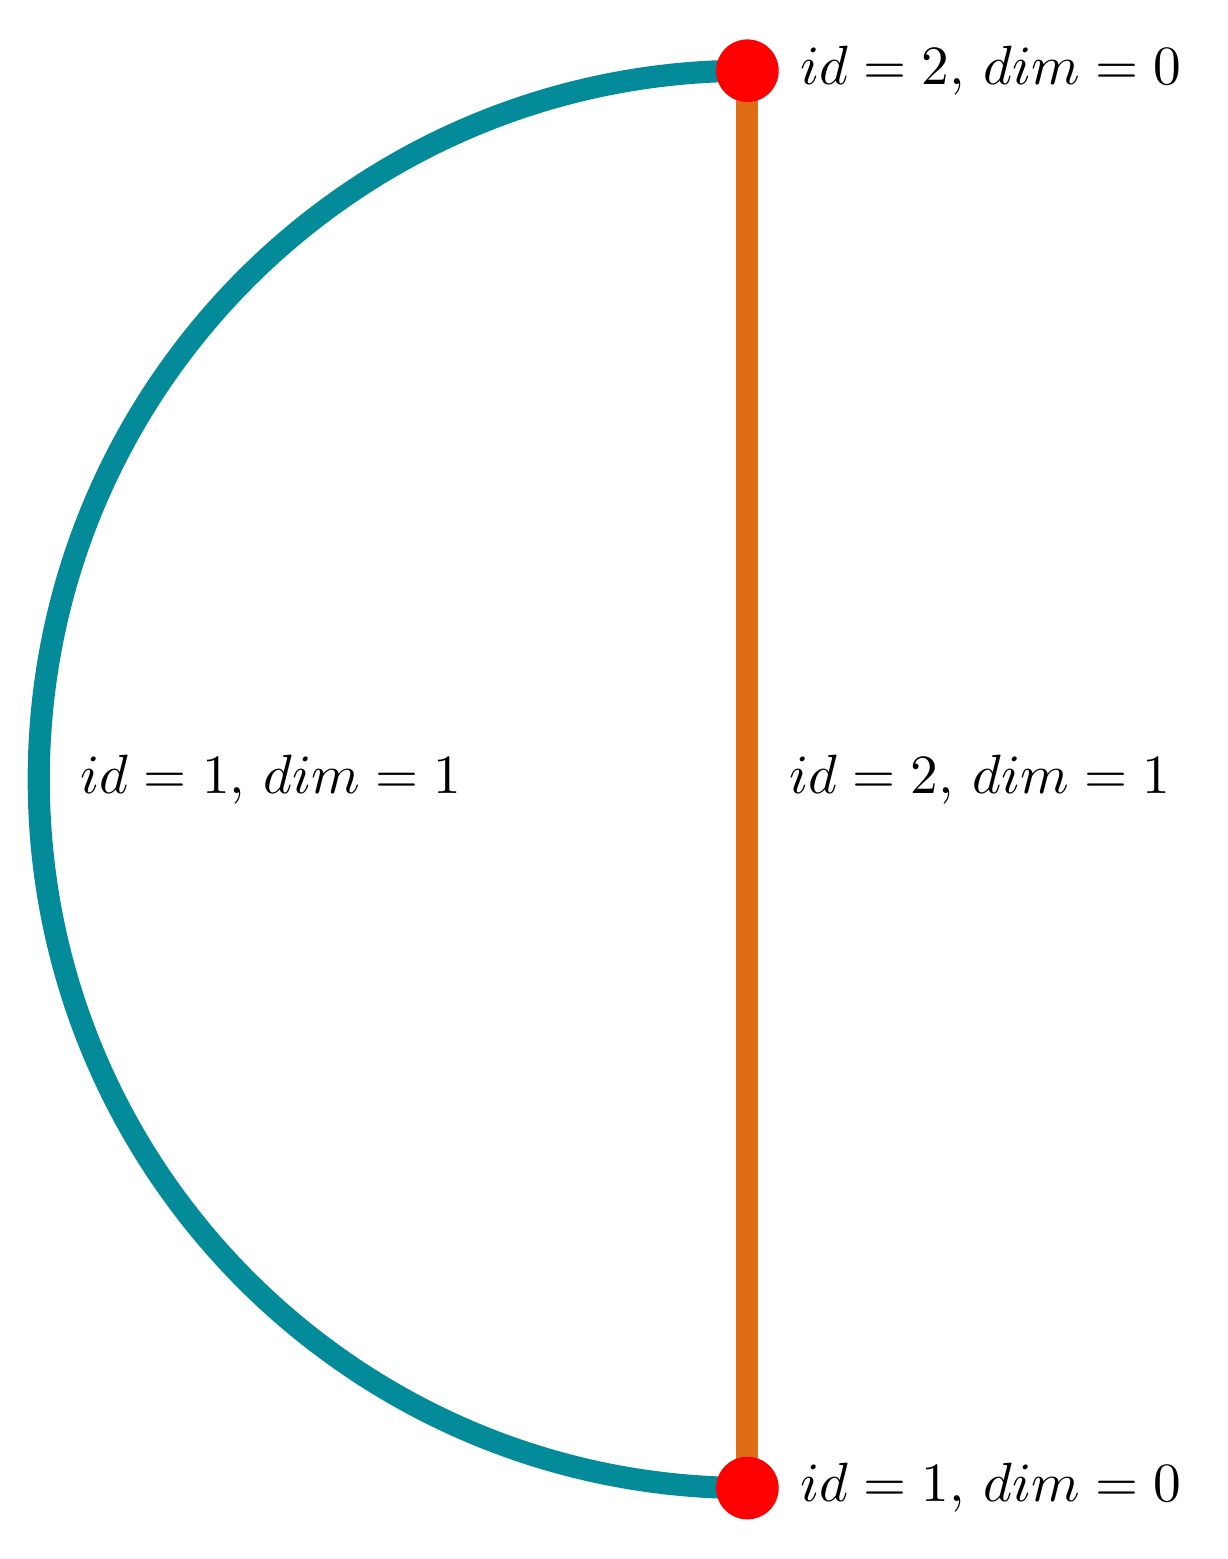
\begin{tikzpicture}

  % Bounding box of the scheme
  \draw (-4,0) node (Bb1) {} ;
  \draw (0,0) node (Bb2) {} ;

  %%%%%%%%%%%%%%%%%%%%%%%%%%%%%%%%% Background of the mesh %%%%%%%%%%%%%%%%%%%%%%%%%%%%%%%%%%%%
  \draw[color=cccanard, line width=8] (0,9) arc [start angle=90, end angle=270, x radius=9cm, y radius=9cm];
  \draw[color=cccitrouille, line width=8] (0,9) -- (0,-9) ;
  
  %%%%%%%%%%%%%%%%%%%%%%%%%%%%%%%%% Points pour travailler %%%%%%%%%%%%%%%%%%%%%%%%%%%%%%%%%%%%

  % Sommets de blocs
 \draw (0,-9) node[circle, fill=red, inner sep=8pt] (2) {} ;
 \draw (0,9) node[circle, fill=red, inner sep=8pt] (3) {} ;

 \draw (2) node[scale=2, right = 6pt] {$id=1$, $dim=0$} ;
 \draw (3) node[scale=2, right = 6pt] {$id=2$, $dim=0$} ;

 \draw (-9,0) node[scale=2, right = 4pt] {$id=1$, $dim=1$} ;
 \draw (0,0) node[scale=2, right = 4pt] {$id=2$, $dim=1$} ;
 

\end{tikzpicture}
\end{document}
